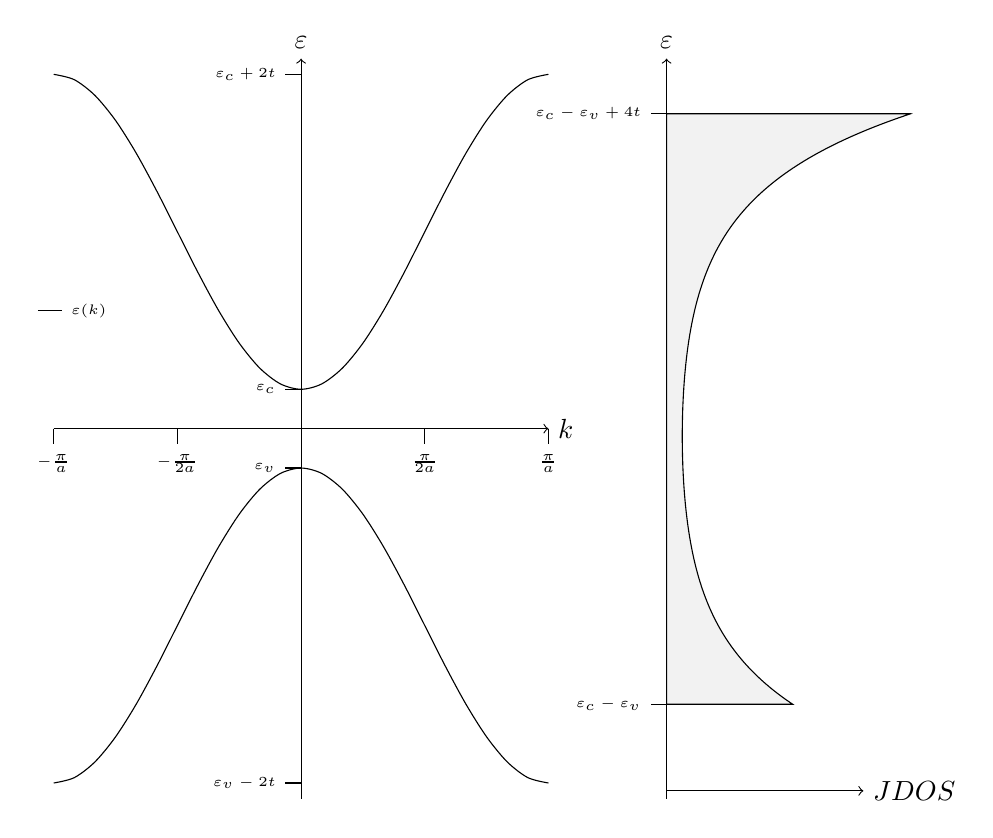
\begin{tikzpicture}
    % Axes
    \draw[->] (-pi,0) -- (pi,0) node[right] {$k$};
    \draw[->] (0,-4.7) -- (0,4.7) node[above] {$\varepsilon$};
    
    % Ticks
        %y
        \draw (0,4.5) -- (-0.2,4.5) node[left] {\tiny{$\varepsilon_c + 2t$}};
        \draw (0,0.5) -- (-0.2,0.5) node[left] {\tiny{$\varepsilon_c$}};
        \draw (0,-0.5) -- (-0.2,-0.5) node[left] {\tiny{$\varepsilon_v$}};
        \draw (0,-4.5) -- (-0.2,-4.5) node[left] {\tiny{$\varepsilon_v-2t$}};
        
        %x
        \draw (-pi,0)   -- (-pi,-0.2)    node[below] {\tiny{$-\frac{\pi}{a}$}};
        \draw (-pi/2,0) -- (-pi/2,-0.2)  node[below] {\tiny{$-\frac{\pi}{2a}$}};
        \draw (pi/2,0)  -- (pi/2,-0.2)   node[below] {\tiny{$\frac{\pi}{2a}$}};
        \draw (pi,0)    -- (pi,-0.2)     node[below] {\tiny{$\frac{\pi}{a}$}};
    
    % Legend
    \draw (-pi-0.2,1.5) -- (-pi+0.1,1.5) node[right] {\tiny{$\varepsilon(k)$}};
    
    
    % Bands
    \draw[color=black,smooth,domain=-pi:pi]  plot (\x,{2.5-2*cos(\x r)});
    \draw[color=black,smooth,domain=-pi:pi]  plot (\x,{-(2.5-2*cos(\x r))});
    
    
    
    % Axes for JDOS
    \draw[->] (pi+1.5,-4.6) -- (pi + 4,-4.6) node[right] {$JDOS$};
    \draw[->] (pi+1.5,-4.7) -- (pi+1.5,4.7) node[above] {$\varepsilon$};
    
    
    %Ticks for JDOS
    \draw (pi+1.5,-3.5) -- (pi+1.3,-3.5) node[left] {\tiny{$\varepsilon_c -\varepsilon_v$}};
    \draw (pi+1.5,4) -- (pi+1.3,4) node[left] {\tiny{$\varepsilon_c -\varepsilon_v + 4t$}};
    
    
    % JDOS
    %\filldraw[color=black,fill=black!5!white,smooth,samples=1000,variable=\y,domain=-3.5:0.5] (pi+1.5,-3.5) -- (pi+2.75,-3.5) -- plot ({pi+1.6+1.15*exp(-(\y+3.5))},{\y}) -- (pi+1.5,4.5) -- (pi+4,4.5);
    \filldraw[color=black,fill=black!5!white,smooth,samples=1000,variable=\y,domain=-3.5:4] (pi+1.5,-3.5) -- (pi+2.75,-3.5) -- plot ({1.5*exp(-(\y+3.5))+pi+1.6+3*exp(-(4-\y))},{\y}) -- (pi+1.6+3,4) -- (pi+1.5,4) -- (pi+1.5,-3.5);
    
\end{tikzpicture}
%{-(1/2)/(sqrt(abs(1-(\y+3.5)*(\y-4.5)/4)))}